\RequirePackage[l2tabu, orthodox]{nag}

%\documentclass[]{article}
\documentclass[11pt]{scrartcl}
\usepackage[usename, dvipsnames]{xcolor}
\usepackage[pdfencoding=auto]{hyperref}
\usepackage[msc-links]{amsrefs}
\usepackage{cleveref} % use \cref{}, automatically deduces theorem, proposition, etc
\usepackage[mathletters]{ucs}
\usepackage[utf8]{inputenc}
\usepackage[T1]{fontenc}
\usepackage{datetime}

\usepackage{array}
\usepackage{mathtools}
\usepackage{amsmath, amsthm, amssymb, amsfonts, amsxtra, amscd, thmtools}
\let\proof\relax
\let\endproof\relax

% Boxes around theorem environments.
\usepackage[many]{tcolorbox}

\usepackage{color}
%\usepackage{unicode-math}
\usepackage{newunicodechar}
\newunicodechar{ε}{\varepsilon}
\newunicodechar{δ}{\delta}
\newunicodechar{µ}{\mu}
\newunicodechar{→}{\to}
\newunicodechar{≤}{\leq}
\newunicodechar{∈}{\in}
\newunicodechar{⊆}{\subseteq}
\newunicodechar{Λ}{\Lambda}
\newunicodechar{∞}{\infty}
\newunicodechar{×}{\times}
\everymath{\displaystyle}



\usepackage{microtype}
\usepackage[pdfencoding=auto]{hyperref}
\usepackage{bookmark}
\usepackage{booktabs}
\usepackage{todonotes}
\usepackage[msc-links]{amsrefs}
\usepackage{cleveref} % use \cref{}, automatically deduces theorem, proposition, etc
\usepackage{csquotes}
\usepackage{longtable}
\usepackage{tabularx}
\usepackage{bbm}
% Creating multiple types of index
\usepackage{imakeidx}

% Remove indentation for new paragraphs
\usepackage{parskip}
% But leave space before amsthm environments
\makeatletter
\def\thm@space@setup{%
  \thm@preskip=2em
  \thm@postskip=2em
}
\makeatother


\usepackage{stmaryrd}
\usepackage{adjustbox}
\usepackage{centernot}
% \centernot\whatever


% Better indicator function
\usepackage{bbm}
\newcommand{\indic}[1]{\mathbbm{1} \left[ {#1} \right] }

% Highlight quote
\usepackage{environ}
\definecolor{camel}{rgb}{0.76, 0.6, 0.42}
\definecolor{babyblue}{rgb}{0.54, 0.81, 0.94}
\definecolor{block-gray}{gray}{0.85}
\NewEnviron{myblock}
{\colorbox{block-gray}{%
\parbox{\dimexpr\linewidth-2\fboxsep\relax}{%
\small\addtolength{\leftskip}{10mm}
\addtolength{\rightskip}{10mm}
\BODY}}
}
\renewcommand{\quote}{\myblock}
\renewcommand{\endquote}{\endmyblock}

% Nice math font that journals use
%\usepackage[lite]{mtpro2}
%\usepackage{mathrsfs}
%\usepackage{mathptmx}
\usepackage{lmodern}
%\usepackage[sc]{mathpazo}

% Theorem Styles
\usepackage[framemethod=tikz]{mdframed}

\theoremstyle{definition}
\newtheorem{exercise}{Exercise}[section]
\newtheorem{solution}{Solution}

% Theorem Style
\newtheoremstyle{theorem}% name
  {0em}%         Space above, empty = `usual value'
  {1em}%         Space below
  {\normalfont}% Body font
  {\parindent}%         Indent amount (empty = no indent, \parindent = para indent)
  {\bfseries}% Thm head font
  {.}%        Punctuation after thm head
  {\newline}% Space after thm head: \newline = linebreak
  {\thmname{#1}\thmnumber{ #2}\thmnote{\itshape{(#3)}}}%
\theoremstyle{theorem}
\tcolorboxenvironment{theorem}{
  boxrule=0pt,
  boxsep=0pt,
  breakable,
  enhanced jigsaw,
  fonttitle={\large\bfseries},
  opacityback=0.8,
  colframe=cyan,
  borderline west={4pt}{0pt}{orange},
  attach title to upper={}
}
\newtheorem{theorem}{Theorem}[section]

% Proposition Style
\tcolorboxenvironment{proposition}{
  boxrule=1pt,
  boxsep=0pt,
  breakable,
  enhanced jigsaw,
  opacityback=0.0,
  colframe=cyan
}
\newtheorem{proposition}[theorem]{Proposition}
\tcolorboxenvironment{lemma}{
  boxrule=1pt,
  boxsep=0pt,
  breakable,
  enhanced jigsaw,
  opacityback=0.2,
  colframe=cyan
}
\newtheorem{lemma}[theorem]{Lemma}
% Claim
\tcolorboxenvironment{claim}{
  boxrule=1pt,
  boxsep=0pt,
  breakable,
  enhanced jigsaw,
  opacityback=0.2,
  colframe=cyan
}
\newtheorem{claim}[theorem]{Claim}


% Corollary
\tcolorboxenvironment{corollary}{
  colback=cyan,
  boxrule=1pt,
  boxsep=0pt,
  breakable,
  enhanced jigsaw,
  opacityback=0.1,
  colframe=cyan
}
\newtheorem{corollary}[theorem]{Corollary}

% Proof Style
\newtheoremstyle{proof}% name
  {0em}%         Space above, empty = `usual value'
  {2em}%         Space below
  {\normalfont}% Body font
  {\parindent}%         Indent amount (empty = no indent, \parindent = para indent)
  {\itshape}% Thm head font
  {.}%        Punctuation after thm head
  {\newline}% Space after thm head: \newline = linebreak
  {\thmname{#1} \thmnote{\itshape{(#3)}}}%         Thm head spec
\theoremstyle{proof}
\tcolorboxenvironment{proof}{
  colback=camel,
  opacityfill=0.25,
  boxrule=1pt,
  boxsep=0pt,
  breakable,
  enhanced jigsaw
}
\newtheorem*{pf}{Proof}
\newenvironment{proof}
{\pushQED{$\qed$}\pf}
{\par\popQED\endpf}

% Definition Style
\newtheoremstyle{definition}% name
  {0em}%         Space above, empty = `usual value'
  {2em}%         Space below
  {\normalfont}% Body font
  {\parindent}%         Indent amount (empty = no indent, \parindent = para indent)
  {\bfseries}% Thm head font
  {.}%        Punctuation after thm head
  {\newline}% Space after thm head: \newline = linebreak
  {}%         Thm head spec
\theoremstyle{definition}
\tcolorboxenvironment{definition}{
  colback=babyblue,
  boxrule=0pt,
  boxsep=0pt,
  opacityfill=0.45,
  breakable,
  enhanced jigsaw,
  borderline west={4pt}{0pt}{blue},
  colbacktitle={babyblue},
  coltitle={black},
  fonttitle={\large\bfseries},
  attach title to upper={},
}
\newtheorem{definition}{Definition}[theorem]

% Break Environment
\makeatletter
\newtheoremstyle{break}% name
  {}%         Space above, empty = `usual value'
  {2em}%         Space below
  {
    \addtolength{\@totalleftmargin}{2.5em}
    \addtolength{\linewidth}{-2.5em}
    \parshape 1 2.5em \linewidth
  }% Body font
  {}%         Indent amount (empty = no indent, \parindent = para indent)
  {\bfseries}% Thm head font
  {.}%        Punctuation after thm head
  {\newline}% Space after thm head: \newline = linebreak
  {}%         Thm head spec
\makeatother

\theoremstyle{break}
\newtheorem{example}{Example}[section]

% Problem Style
\newtheoremstyle{problem} % name
  {0em}                   % Space above, empty = `usual value'
  {2em}                   % Space below
  {\normalfont}           % Body font
  {\parindent}            % Indent amount (empty = no indent, \parindent = para indent)
  {\itshape}              % Thm head font
  {}                      % Punctuation after thm head
  {\newline}              % Space after thm head: \newline = linebreak
  {\thmnote{\itshape{(#3)}}}     % Thm head spec
\theoremstyle{problem}
\tcolorboxenvironment{problem}{
  boxrule=1pt,
  boxsep=0pt,
  breakable,
  enhanced jigsaw,
  opacityback=0.0,
  colframe=cyan
}
\newtheorem{problem}{Problem}


%Pagination stuff.
\setlength{\topmargin}{-.3 in}
\setlength{\oddsidemargin}{0in}
\setlength{\evensidemargin}{0in}
\setlength{\textheight}{9.in}
\setlength{\textwidth}{6.5in}
% \pagestyle{empty} %removes page numbers.

% Inkscape figures from Vim
\usepackage{import}
\usepackage{pdfpages}
\usepackage{transparent}

\newcommand{\incfig}[1]{%
    \def\svgwidth{\columnwidth}
    \import{./figures/}{#1.pdf_tex}
}
%\pdfsuppresswarningpagegroup=1

% Pandoc-specific fixes
\providecommand{\tightlist}{%
  \setlength{\itemsep}{0pt}\setlength{\parskip}{0pt}}

% Tikz and Graphics
\usepackage{amscd}
\usepackage{tikz}
\usetikzlibrary{arrows, arrows.meta, cd, fadings, patterns, calc, decorations.markings, matrix, positioning}
\tikzfading[name=fade out, inner color=transparent!0, outer color=transparent!100]
\usepackage{pgfplots}
\pgfplotsset{compat=1.16}
\usepackage[inline]{asymptote}
\usepackage{tikz-layers}

%\usepackage{nath}
%\delimgrowth=1
\DeclarePairedDelimiter\qty{(}{)}

% Major Macros
\usepackage{graphicx}
\usepackage{float}
\DeclareFontFamily{U}{mathx}{\hyphenchar\font45}
\DeclareFontShape{U}{mathx}{m}{n}{
      <5> <6> <7> <8> <9> <10>
      <10.95> <12> <14.4> <17.28> <20.74> <24.88>
      mathx10
      }{}
\DeclareSymbolFont{mathx}{U}{mathx}{m}{n}
\DeclareMathSymbol{\bigtimes}{1}{mathx}{"91}

% Wide tikz equations
\newsavebox{\wideeqbox}
\newenvironment{wideeq}
  {\begin{displaymath}\begin{lrbox}{\wideeqbox}$\displaystyle}
  {$\end{lrbox}\makebox[0pt]{\usebox{\wideeqbox}}\end{displaymath}}



% Fancy chapter headers and footers
\usepackage{fancyhdr}

\pagestyle{fancy}
\fancyhf{}
\fancyhead[LE,RO]{\title}
\fancyhead[RE,LO]{\rightmark}
\fancyfoot[CE,CO]{\leftmark}
\fancyfoot[LE,RO]{\thepage}

\renewcommand{\headrulewidth}{2pt}
\renewcommand{\footrulewidth}{1pt}

% List of Theorems Attempt
\usepackage{etoolbox}
\makeatletter
\patchcmd\thmtlo@chaptervspacehack
  {\addtocontents{loe}{\protect\addvspace{10\p@}}}
  {\addtocontents{loe}{\protect\thmlopatch@endchapter\protect\thmlopatch@chapter{\thechapter}}}
  {}{}
\AtEndDocument{\addtocontents{loe}{\protect\thmlopatch@endchapter}}
\long\def\thmlopatch@chapter#1#2\thmlopatch@endchapter{%
  \setbox\z@=\vbox{#2}%
  \ifdim\ht\z@>\z@
    \hbox{\bfseries\chaptername\ #1}\nobreak
    #2
    \addvspace{10\p@}
  \fi
}
\def\thmlopatch@endchapter{}

\makeatother
\renewcommand{\thmtformatoptarg}[1]{ -- #1}
%\renewcommand{\listtheoremname}{List of definitions}

\newcommand{\ext}{\operatorname{Ext}}
\newcommand{\Ext}{\operatorname{Ext}}
\def\Endo{\operatorname{End}}
\def\Ind{\operatorname{Ind}}
\def\ind{\operatorname{Ind}}
\def\coind{\operatorname{Coind}}
\def\Res{\operatorname{Res}}
\def\Hol{\operatorname{Hol}}
\def\res{\operatorname{Res}}
\def\endo{\operatorname{End}}
\def\ind{\operatorname{Ind}}
\renewcommand{\AA}[0]{{\mathbb{A}}}
\DeclareMathOperator{\Exists}{\exists}
\DeclareMathOperator{\Forall}{\forall}
\newcommand{\Af}[0]{{\mathbb{A}}}
\newcommand{\CC}[0]{{\mathbb{C}}}
\newcommand{\CP}[0]{{\mathbb{CP}}}
\newcommand{\DD}[0]{{\mathbb{D}}}
\newcommand{\FF}[0]{{\mathbb{F}}}
\newcommand{\GF}[0]{{\mathbb{GF}}}
\newcommand{\GG}[0]{{\mathbb{G}}}
\newcommand{\HH}[0]{{\mathbb{H}}}
\newcommand{\HP}[0]{{\mathbb{HP}}}
\newcommand{\KK}[0]{{\mathbb{K}}}
\newcommand{\kk}[0]{{\Bbbk}}
\newcommand{\bbm}[0]{{\mathbb{M}}}
\newcommand{\NN}[0]{{\mathbb{N}}}
\newcommand{\OP}[0]{{\mathbb{OP}}}
\newcommand{\PP}[0]{{\mathbb{P}}}
\newcommand{\QQ}[0]{{\mathbb{Q}}}
\newcommand{\RP}[0]{{\mathbb{RP}}}
\newcommand{\RR}[0]{{\mathbb{R}}}
\newcommand{\SpSp}[0]{{\mathbb{S}}}
\renewcommand{\SS}[0]{{\mathbb{S}}}
\newcommand{\TT}[0]{{\mathbb{T}}}
\newcommand{\ZZ}[0]{{\mathbb{Z}}}
\newcommand{\ZnZ}[0]{\mathbb{Z}/n\mathbb{Z}}
\newcommand{\ZpZ}[0]{\mathbb{Z}/p\mathbb{Z}}
\newcommand{\Qp}[0]{\mathbb{Q}_{(p)}}
\newcommand{\Zp}[0]{\mathbb{Z}_{(p)}}
\newcommand{\Arg}[0]{\mathrm{Arg}}
\newcommand{\PGL}[0]{\mathrm{PGL}}
\newcommand{\GL}[0]{\mathrm{GL}}
\newcommand{\Gl}[0]{\mathrm{GL}}
\newcommand{\gl}[0]{\mathrm{GL}}
\newcommand{\mat}[0]{\mathrm{Mat}}
\newcommand{\Mat}[0]{\mathrm{Mat}}
\newcommand{\Rat}[0]{\mathrm{Rat}}
\newcommand{\Perv}[0]{\mathrm{Perv}}
\newcommand{\Gal}[0]{\mathrm{Gal}}
\newcommand{\Hilb}[0]{\mathrm{Hilb}}
\newcommand{\Quot}[0]{\mathrm{Quot}}
\newcommand{\Art}[0]{\mathrm{Art}}
\newcommand{\red}[0]{\mathrm{red}}
\newcommand{\alg}[0]{\mathrm{alg}}
\newcommand{\Pic}[0]{{\mathrm{Pic}~}}
\newcommand{\lcm}[0]{\mathrm{lcm}}
\newcommand{\maps}[0]{\mathrm{Maps}}
\newcommand{\maxspec}[0]{{\mathrm{maxSpec}~}}
\newcommand{\Tr}[0]{\mathrm{Tr}}
\newcommand{\adj}[0]{\mathrm{adj}}
\newcommand{\ad}[0]{\mathrm{ad}~}
\newcommand{\ann}[0]{\mathrm{Ann}}
\newcommand{\Ann}[0]{\mathrm{Ann}}
\newcommand{\arcsec}[0]{\mathrm{arcsec}}
\newcommand{\ch}[0]{\mathrm{char}~}
\newcommand{\Sp}[0]{{\mathrm{Sp}}}
\newcommand{\syl}[0]{{\mathrm{Syl}}}
\newcommand{\txand}[0]{{\text{ and }}}
\newcommand{\codim}[0]{\mathrm{codim}}
\newcommand{\txor}[0]{{\text{ or }}}
\newcommand{\txt}[1]{{\text{ {#1} }}}
\newcommand{\Gr}[0]{{\text{Gr}}}
\newcommand{\Aut}[0]{{\mathrm{Aut}}}
\newcommand{\aut}[0]{\mathrm{Aut}}
\newcommand{\Inn}[0]{{\mathrm{Inn}}}
\newcommand{\Out}[0]{{\mathrm{Out}}}
\newcommand{\mltext}[1]{\left\{\begin{array}{c}#1\end{array}\right\}}
\newcommand{\Fun}[0]{{\text{Fun}}}
\newcommand{\SL}[0]{{\text{SL}}}
\newcommand{\PSL}[0]{{\text{PSL}}}
\newcommand{\SO}[0]{{\text{SO}}}
\newcommand{\SU}[0]{{\text{SU}}}
\newcommand{\SP}[0]{{\text{SP}}}
\newcommand{\per}[0]{{\text{Per}}}
\newcommand{\loc}[0]{{\text{loc}}}
\newcommand{\Top}[0]{{\text{Top}}}
\newcommand{\Sch}[0]{{\text{Sch}}}
\newcommand{\sch}[0]{{\text{Sch}}}
\newcommand{\Set}[0]{{\text{Set}}}
\newcommand{\Sets}[0]{{\text{Set}}}
\newcommand{\Grp}[0]{{\text{Grp}}}
\newcommand{\Groups}[0]{{\text{Groups}}}
\newcommand{\Homeo}[0]{{\text{Homeo}}}
\newcommand{\Diffeo}[0]{{\text{Diffeo}}}
\newcommand{\MCG}[0]{{\text{MCG}}}
\newcommand{\set}[0]{{\text{Set}}}
\newcommand{\Tor}[0]{\text{Tor}}
\newcommand{\sets}[0]{{\text{Set}}}
\newcommand{\Sm}[0]{{\text{Sm}_k}}
\newcommand{\orr}[0]{{\text{ or }}}
\newcommand{\annd}[0]{{\text{ and }}}
\newcommand{\bung}[0]{\text{Bun}_G}
\newcommand{\const}[0]{{\text{const.}}}
\newcommand{\disc}[0]{{\text{disc}}}
\newcommand{\op}[0]{^\text{op}}
\newcommand{\id}[0]{\text{id}}
\newcommand{\im}[1]{\mathrm{im}({#1})}
\newcommand{\pt}[0]{{\{\text{pt}\}}}
\newcommand{\sep}[0]{^\text{sep}}
% \newcommand{\st}[0]{~{\text{s.t.}}~}
\newcommand{\tors}[0]{{\text{tors}}}
\newcommand{\tor}[0]{\text{Tor}}
\newcommand{\height}[0]{\text{ht}}
\newcommand{\cpt}[0]{\text{compact}}
\newcommand{\abs}[1]{{\left\lvert {#1} \right\rvert}}
\newcommand{\stack}[1]{\mathclap{\substack{ #1 }}} 
\newcommand{\qtext}[1]{{\quad \text{#1} \quad}}
\newcommand{\qst}[0]{{\quad \text{such that} \quad}}
\newcommand{\actsonl}[0]{\curvearrowleft}
\newcommand{\actson}[0]{\curvearrowright}
\newcommand{\bd}[0]{{\del}}
\newcommand{\bigast}[0]{{\mathop{\Large \ast}}}
\newcommand{\coker}[0]{\operatorname{coker}}
\newcommand{\cok}[0]{\operatorname{coker}}
\newcommand{\conjugate}[1]{{\overline{{#1}}}}
\newcommand{\converges}[1]{\overset{#1}}
\newcommand{\correspond}[1]{\theset{\substack{#1}}}
\newcommand{\cross}[0]{\times}
\newcommand{\by}[0]{\times}
\newcommand{\dash}[0]{{\hbox{-}}}
\newcommand{\dd}[2]{{\frac{\partial #1}{\partial #2}\,}}
\newcommand{\definedas}[0]{\coloneqq}
\newcommand{\da}[0]{\coloneqq}
\newcommand{\del}[0]{{\partial}}
\newcommand{\directlim}[0]{\varinjlim}
\newcommand{\disjoint}[0]{{\coprod}}
\newcommand{\divides}[0]{{~\Bigm|~}}
\newcommand{\dual}[0]{^\vee}
\newcommand{\sm}[0]{\setminus}
\newcommand{\smz}[0]{\setminus\theset{0}}
\newcommand{\eps}[0]{\varepsilon}
\newcommand{\equalsbecause}[1] {\stackrel{\mathclap{\scriptscriptstyle{#1}}}{=}}
\newcommand{\floor}[1]{{\left\lfloor #1 \right\rfloor}}
\DeclarePairedDelimiter{\ceil}{\lceil}{\rceil}
\newcommand{\from}[0]{\leftarrow}
\newcommand{\tofrom}[0]{\leftrightarrows}
\newcommand{\up}[0]{\uparrow}
\newcommand{\generators}[1]{\left\langle{#1}\right\rangle}
\newcommand{\gs}[1]{\left\langle{#1}\right\rangle}
\newcommand{\homotopic}[0]{\simeq}
\newcommand{\injectivelim}[0]{\varinjlim}
\newcommand{\injects}[0]{\hookrightarrow}
\newcommand{\inner}[2]{{\left\langle {#1},~{#2} \right\rangle}}
\newcommand{\union}[0]{\cup}
\newcommand{\Union}[0]{\bigcup}
\newcommand{\intersect}[0]{\cap}
\newcommand{\Intersect}[0]{\bigcap}
\newcommand{\into}[0]{\to}
\newcommand{\inverselim}[0]{\varprojlim}
\newcommand{\inv}[0]{^{-1}}
\newcommand{\mfa}[0]{{\mathfrak{a}}}
\newcommand{\mfb}[0]{{\mathfrak{b}}}
\newcommand{\mfc}[0]{{\mathfrak{c}}}
\newcommand{\mff}[0]{{\mathfrak{f}}}
\newcommand{\mfi}[0]{{\mathfrak{I}}}
\newcommand{\mfm}[0]{{\mathfrak{m}}}
\newcommand{\mfn}[0]{{\mathfrak{n}}}
\newcommand{\mfp}[0]{{\mathfrak{p}}}
\newcommand{\mfq}[0]{{\mathfrak{q}}}
\newcommand{\mfr}[0]{{\mathfrak{r}}}
\newcommand{\lieb}[0]{{\mathfrak{b}}}
\newcommand{\liegl}[0]{{\mathfrak{gl}}}
\newcommand{\lieg}[0]{{\mathfrak{g}}}
\newcommand{\lieh}[0]{{\mathfrak{h}}}
\newcommand{\lien}[0]{{\mathfrak{n}}}
\newcommand{\liesl}[0]{{\mathfrak{sl}}}
\newcommand{\lieso}[0]{{\mathfrak{so}}}
\newcommand{\liesp}[0]{{\mathfrak{sp}}}
\newcommand{\lieu}[0]{{\mathfrak{u}}}
\newcommand{\nilrad}[0]{{\mathfrak{N}}}
\newcommand{\jacobsonrad}[0]{{\mathfrak{J}}}
\newcommand{\mm}[0]{{\mathfrak{m}}}
\newcommand{\pr}[0]{{\mathfrak{p}}}
\newcommand{\mapsvia}[1]{\xrightarrow{#1}}
\newcommand{\kx}[1]{k[x_1, \cdots, x_{#1}]}
\newcommand{\MM}[0]{{\mathcal{M}}}
\newcommand{\OO}[0]{{\mathcal{O}}}
\newcommand{\imaginarypart}[1]{{\mathcal{Im}({#1})}}
\newcommand{\mca}[0]{{\mathcal{A}}}
\newcommand{\mcb}[0]{{\mathcal{B}}}
\newcommand{\mcc}[0]{{\mathcal{C}}}
\newcommand{\mcd}[0]{{\mathcal{D}}}
\newcommand{\mce}[0]{{\mathcal{E}}}
\newcommand{\mcf}[0]{{\mathcal{F}}}
\newcommand{\mcg}[0]{{\mathcal{G}}}
\newcommand{\mch}[0]{{\mathcal{H}}}
\newcommand{\mci}[0]{{\mathcal{I}}}
\newcommand{\mcj}[0]{{\mathcal{J}}}
\newcommand{\mck}[0]{{\mathcal{K}}}
\newcommand{\mcl}[0]{{\mathcal{L}}}
\newcommand{\mcm}[0]{{\mathcal{M}}}
\newcommand{\mcp}[0]{{\mathcal{P}}}
\newcommand{\mcs}[0]{{\mathcal{S}}}
\newcommand{\mct}[0]{{\mathcal{T}}}
\newcommand{\mcu}[0]{{\mathcal{U}}}
\newcommand{\mcv}[0]{{\mathcal{V}}}
\newcommand{\mcx}[0]{{\mathcal{X}}}
\newcommand{\mcz}[0]{{\mathcal{Z}}}
\newcommand{\cl}[0]{\mathrm{cl}}
\newcommand{\trdeg}[0]{\mathrm{trdeg}}
\newcommand{\dist}[0]{\mathrm{dist}}
\newcommand{\Dist}[0]{\mathrm{Dist}}
\newcommand{\crit}[0]{\mathrm{crit}}
\newcommand{\diam}[0]{{\mathrm{diam}}}
\newcommand{\gal}[0]{\mathrm{Gal}}
\newcommand{\diff}[0]{\mathrm{Diff}}
\newcommand{\diag}[0]{\mathrm{diag}}
\newcommand{\soc}[0]{\mathrm{Soc}\,}
\newcommand{\hd}[0]{\mathrm{Head}\,}
\newcommand{\grad}[0]{\mathrm{grad}~}
\newcommand{\hilb}[0]{\mathrm{Hilb}}
\newcommand{\minpoly}[0]{{\mathrm{minpoly}}}
\newcommand{\Hom}[0]{{\mathrm{Hom}}}
\newcommand{\Map}[0]{{\mathrm{Map}}}
\newcommand{\multinomial}[1]{\left(\!\!{#1}\!\!\right)}
\newcommand{\nil}[0]{{\mathrm{nil}}}
\newcommand{\normalneq}{\mathrel{\reflectbox{$\trianglerightneq$}}}
\newcommand{\normal}[0]{{~\trianglelefteq~}}
\newcommand{\norm}[1]{{\left\lVert {#1} \right\rVert}}
\newcommand{\pnorm}[2]{{\left\lVert {#1} \right\rVert}_{#2}}
\newcommand{\notdivides}[0]{\nmid}
\newcommand{\onto}[0]{\twoheadhthtarrow}
\newcommand{\ord}[0]{{\mathrm{Ord}}}
\newcommand{\pic}[0]{{\mathrm{Pic}~}}
\newcommand{\projectivelim}[0]{\varprojlim}
\newcommand{\rad}[0]{{\mathrm{rad}~}}
\newcommand{\ralg}[0]{\mathrm{R-alg}}
\newcommand{\kalg}[0]{k\dash\mathrm{alg}}
\newcommand{\rank}[0]{\operatorname{rank}}
\newcommand{\realpart}[1]{{\mathcal{Re}({#1})}}
\newcommand{\Log}[0]{\mathrm{Log}}
\newcommand{\reg}[0]{\mathrm{Reg}}
\newcommand{\restrictionof}[2]{{\left.{#1}\right|_{#2}}}
\newcommand{\ro}[2]{{\left.{#1}\right|_{#2}}}
\newcommand{\rk}[0]{{\mathrm{rank}}}
\newcommand{\evalfrom}[0]{\Big|}
\newcommand{\rmod}[0]{{R\dash\mathrm{mod}}}
\newcommand{\Mod}[0]{{\mathrm{Mod}}}
\newcommand{\rotate}[2]{{\style{display: inline-block; transform: rotate(#1deg)}{#2}}}
\newcommand{\selfmap}[0]{{\circlearrowleft}}
\newcommand{\semidirect}[0]{\rtimes}
\newcommand{\sgn}[0]{\mathrm{sgn}}
\newcommand{\sign}[0]{\mathrm{sign}}
\newcommand{\spanof}[0]{{\mathrm{span}}}
\newcommand{\spec}[0]{\mathrm{Spec}\,}
\newcommand{\mspec}[0]{\mathrm{mSpec}~}
\newcommand{\stab}[0]{{\mathrm{Stab}}}
\newcommand{\stirlingfirst}[2]{\genfrac{[}{]}{0pt}{}{#1}{#2}}
\newcommand{\stirling}[2]{\genfrac\{\}{0pt}{}{#1}{#2}}
\newcommand{\strike}[1]{{\enclose{horizontalstrike}{#1}}}
\newcommand{\suchthat}[0]{{~\mathrel{\Big|}~}}
\newcommand{\st}[0]{{~\mathrel{\Big|}~}}
\newcommand{\supp}[0]{{\mathrm{supp}}}
\newcommand{\surjects}[0]{\twoheadrightarrow}
\newcommand{\sym}[0]{\mathrm{Sym}}
\newcommand{\tensor}[0]{\otimes}
\newcommand{\connectsum}[0]{\mathop{\Large \#}}
\newcommand{\theset}[1]{\left\{{#1}\right\}}
\newcommand{\ts}[1]{\left\{{#1}\right\}}
\newcommand{\gens}[1]{\left\langle{#1}\right\rangle}
\newcommand{\thevector}[1]{{\left[ {#1} \right]}}
\newcommand{\tv}[1]{{\left[ {#1} \right]}}
\newcommand{\too}[1]{{\xrightarrow{#1}}}
\newcommand{\transverse}[0]{\pitchfork}
\newcommand{\trianglerightneq}{\mathrel{\ooalign{\raisebox{-0.5ex}{\reflectbox{\rotatebox{90}{$\nshortmid$}}}\cr$\triangleright$\cr}\mkern-3mu}}
\newcommand{\tr}[0]{\mathrm{Tr}}
\newcommand{\uniformlyconverges}[0]{\rightrightarrows}
\newcommand{\covers}[0]{\rightrightarrows}
\newcommand{\units}[0]{^{\times}}
\newcommand{\nonzero}[0]{^{\bullet}}
\newcommand{\wait}[0]{{\,\cdot\,}}
\newcommand{\wt}[0]{{\mathrm{wt}}}
\renewcommand{\bar}[1]{\mkern 1.5mu\overline{\mkern-1.5mu#1\mkern-1.5mu}\mkern 1.5mu}
\renewcommand{\div}[0]{\mathrm{Div}}
\newcommand{\Div}[0]{\mathrm{Div}}
\renewcommand{\hat}[1]{\widehat{#1}}
\renewcommand{\mid}[0]{\mathrel{\Big|}}
\renewcommand{\qed}[0]{\hfill\blacksquare}
\renewcommand{\too}[0]{\longrightarrow}
\renewcommand{\vector}[1]{\mathbf{#1}}
\let\oldexp\exp
\renewcommand{\exp}[1]{\oldexp\qty{#1}}
\let\oldperp\perp
\renewcommand{\perp}[0]{^\oldperp}
\newcommand*\dif{\mathop{}\!\mathrm{d}}
\newcommand{\ddt}{\tfrac{\dif}{\dif t}}
\newcommand{\ddx}{\tfrac{\dif}{\dif x}}

\DeclareMathOperator{\righttriplearrows} {{\; \tikz{ \foreach \y in {0, 0.1, 0.2} { \draw [-stealth] (0, \y) -- +(0.5, 0);}} \; }}



\addbibresource{EtaleCohomology.bib}

\let\Begin\begin
\let\End\end
\newcommand\wrapenv[1]{#1}

\makeatletter
\def\ScaleWidthIfNeeded{%
 \ifdim\Gin@nat@width>\linewidth
    \linewidth
  \else
    \Gin@nat@width
  \fi
}
\def\ScaleHeightIfNeeded{%
  \ifdim\Gin@nat@height>0.9\textheight
    0.9\textheight
  \else
    \Gin@nat@width
  \fi
}
\makeatother

\setkeys{Gin}{width=\ScaleWidthIfNeeded,height=\ScaleHeightIfNeeded,keepaspectratio}%

\title{
\rule{\linewidth}{1pt} \\
\textbf{
    Étale Cohomology
  }
    \\ {\normalsize University of Georgia, Fall 2020} \\
  \rule{\linewidth}{2pt}
}
\titlehead{
    \begin{center}
  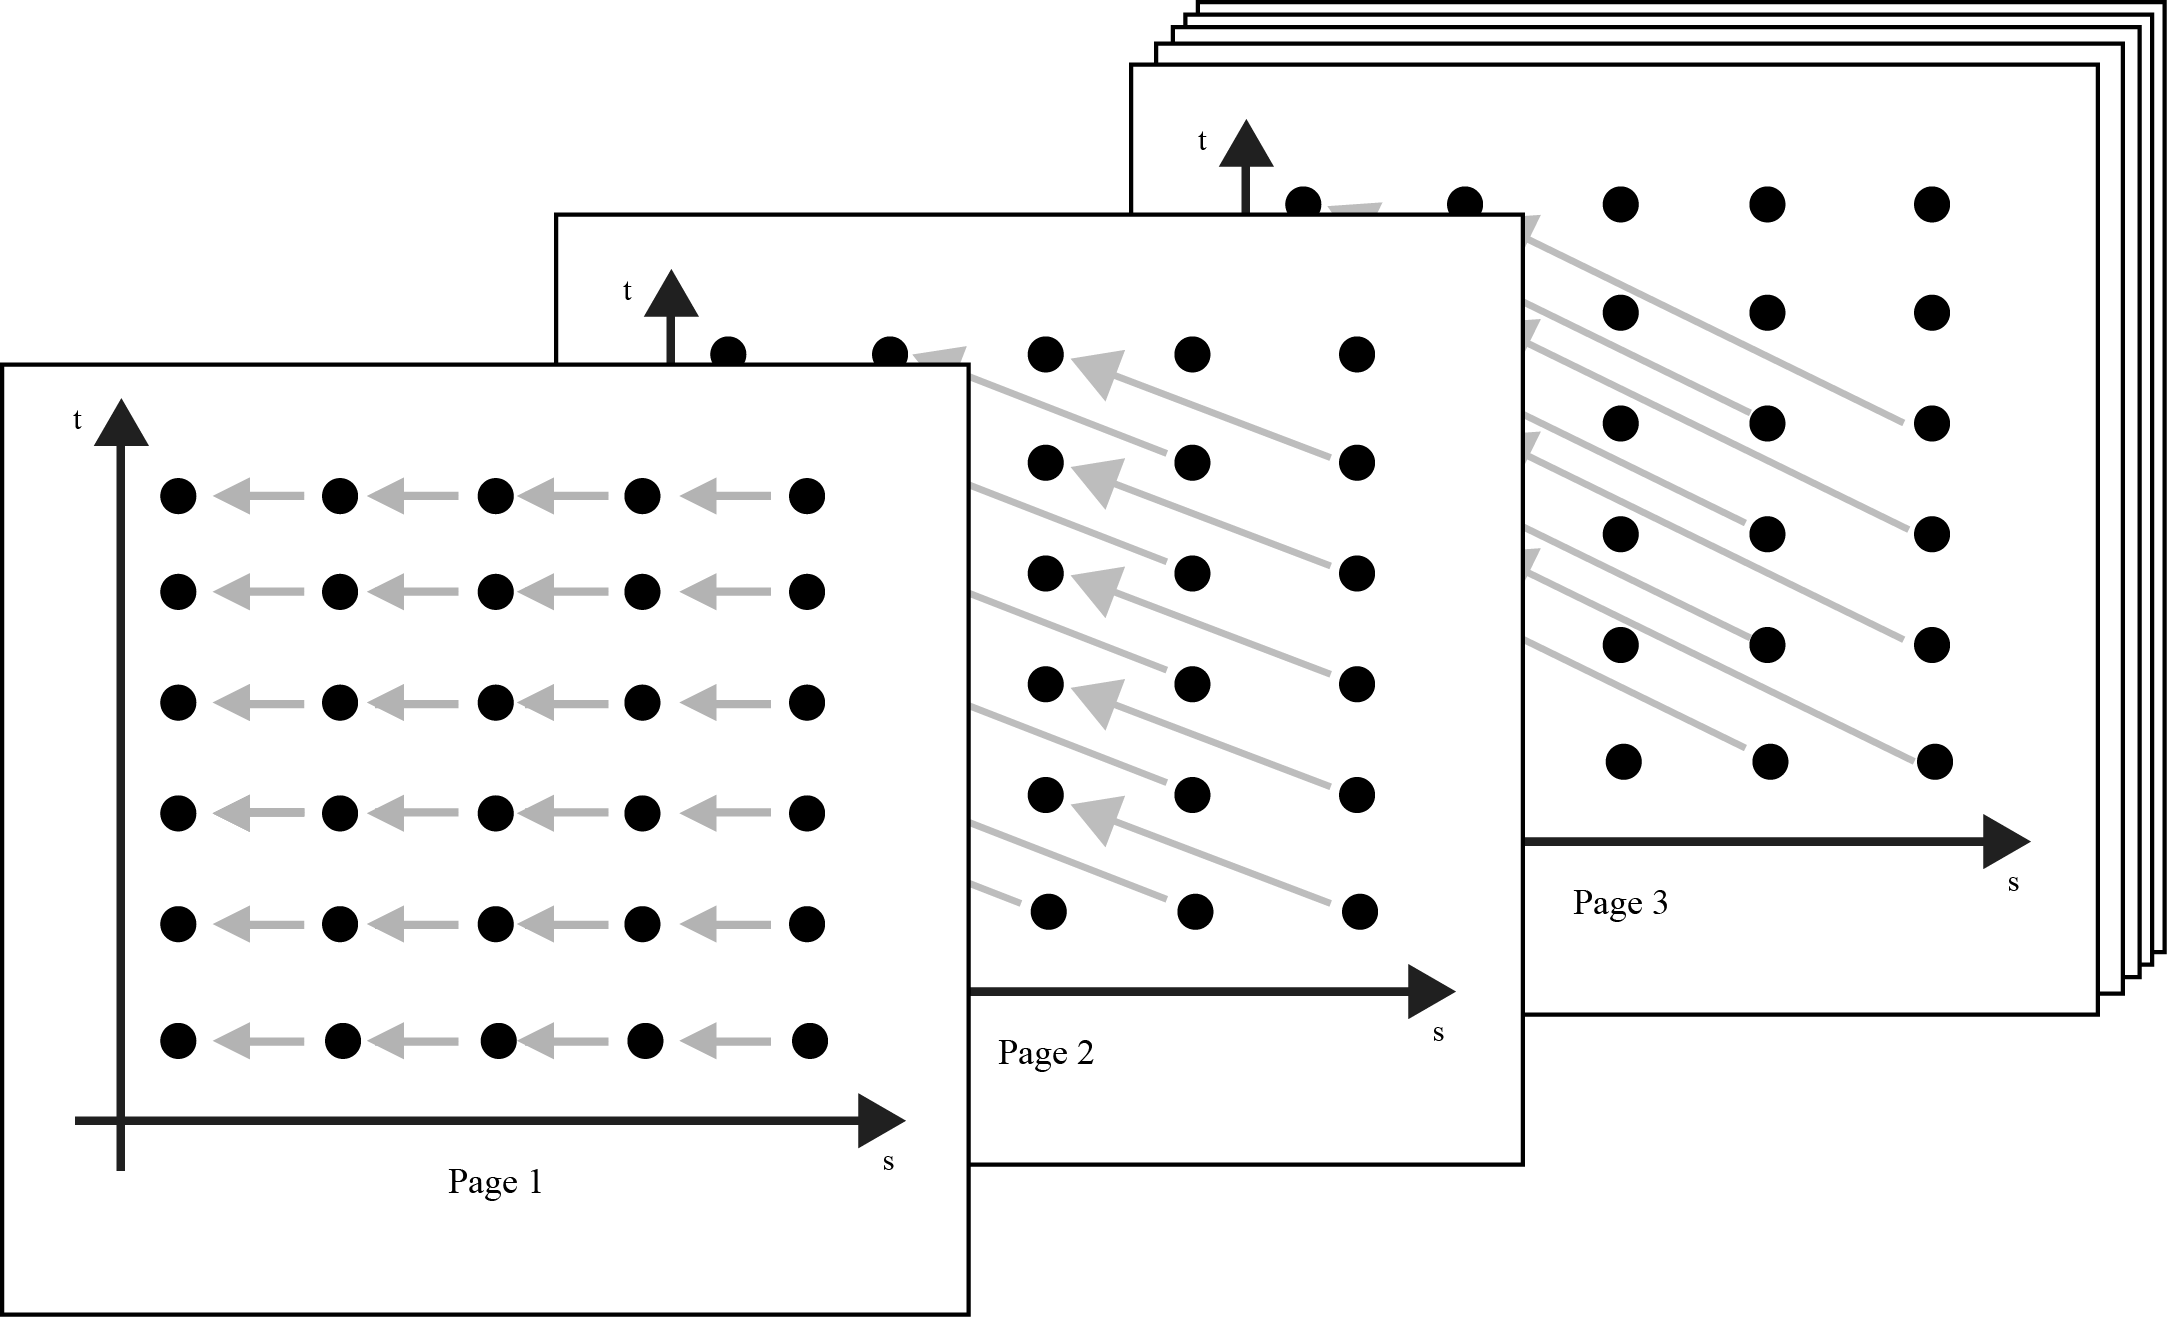
\includegraphics[width=\linewidth,height=0.45\textheight,keepaspectratio]{figures/cover.png}
  \end{center}
       \begin{minipage}{.35\linewidth}
    \begin{flushleft}
      \vspace{2em}
      {\fontsize{6pt}{2pt} \textit{Notes: These are notes live-tex'd
from a graduate course on Étale Cohomology taught by Daniel Litt at the
University of Georgia in Fall 2020. As such, any errors or inaccuracies
are almost certainly my own. } } \\
    \end{flushleft}
    \end{minipage}
    \hfill
    \begin{minipage}{.65\linewidth}
    \end{minipage}
  }







\begin{document}

\date{}
\author{D. Zack Garza}
\maketitle
\begin{flushleft}
\textit{D. Zack Garza} \\
\textit{University of Georgia} \\
  \textit{\href{mailto: dzackgarza@gmail.com}{dzackgarza@gmail.com}} \\
{\tiny \textit{Last updated:} 2020-12-12 }
\end{flushleft}


\newpage

\tableofcontents
\newpage

These are notes live-tex'd from a graduate course in Étale Cohomology
taught by Daniel Litt at the University of Georgia in Fall 2020. As
such, any errors or inaccuracies are almost certainly my own.

\medskip
\begin{flushright}
  D. Zack Garza, \today \\
  \currenttime
\end{flushright}

\hypertarget{lecture-1}{%
\section{Lecture 1}\label{lecture-1}}

\begin{quote}
References: \url{https://www.daniellitt.com/tale-cohomology}
\end{quote}

\hypertarget{intro}{%
\subsection{Intro}\label{intro}}

Prerequisites:

\begin{itemize}
\tightlist
\item
  Homological Algebra

  \begin{itemize}
  \tightlist
  \item
    Abelian Categories
  \item
    Derived Functors
  \item
    Spectral Sequences (just exposure!)
  \end{itemize}
\item
  Sheaf theory and sheaf cohomology
\item
  Schemes (Hartshorne II and III)
\end{itemize}

Outline/Goals:

\begin{itemize}
\tightlist
\item
  Basics of etale cohomology

  \begin{itemize}
  \tightlist
  \item
    Etale morphism
  \item
    Grothendieck topologies
  \item
    The etale topology
  \item
    Etale cohomology and the basis theorems
  \item
    Etale cohomology of curves
  \item
    Comparison theorems to singular cohomology
  \item
    Focused on the case where coefficients are a constructible sheaf.
  \end{itemize}
\item
  Prove the Weil Conjectures (more than one proof)

  \begin{itemize}
  \tightlist
  \item
    Proving the Riemann Hypothesis for varieties over finite fields
  \end{itemize}

  \begin{quote}
  One of the greatest pieces of 20th century mathematics!
  \end{quote}
\item
  Topics

  \begin{itemize}
  \tightlist
  \item
    Weil 2 (Strengthening of RH, used in practice)
  \item
    Formality of algebraic varieties (topological features unique to
    varieties)
  \item
    Other things (monodromy, refer to Katz' AWS notes)
  \end{itemize}
\end{itemize}

\hypertarget{what-is-etale-cohomology}{%
\subsection{What is Etale Cohomology?}\label{what-is-etale-cohomology}}

Suppose \(X/\CC\) is a quasiprojective variety: a finite type separated
integral \(\CC\dash\)scheme.

If you take the complex points, it naturally has the structure of a
complex analytic space \(X(\CC)^{\text{an}}\): you can give it the
Euclidean topology, which is much finer than the Zariski topology.

For a nice topological space, we can associate the singular cohomology
\(H^i(X(\CC)^{\text{an}}, \ZZ)\), which satisfies several nice
properties:

\begin{itemize}
\tightlist
\item
  Finitely generated \(\ZZ\dash\)modules
\item
  Extra Hodge structure when tensored up to \(\CC\) (same as \(\CC\)
  coefficients)
\item
  Cycle classes (i.e.~associate to a subvariety a class in cohomology)
\end{itemize}

Goal of etale cohomology: do something similar for much more general
``nice'' schemes. Note that some of these properties are special to
complex varieties

E.g. finitely generated: not true for a random topological space

We'll associate \(X\) a ``nice scheme''
\(\rightsquigarrow H^i(X_{\text{et}}, \ZZ/\ell^n\ZZ)\). Take the inverse
limit over all \(n\) to obtain the \(\ell\dash\)adic cohomology
\(H^i(X_{\text{et}}, \ZZ_\ell)\). You can tensor with \(\QQ\) to get
something with \(\QQ_\ell\) coefficients. And as in singular cohomology,
you can a ``twisted coefficient system''.

What are nice schemes:

\begin{itemize}
\tightlist
\item
  \(X = \spec \OO_k\), the ring of integers over a number field.
\item
  \(X\) a variety over an algebraically closed field

  \begin{itemize}
  \tightlist
  \item
    Typical, most analogous to taking a variety over \(\CC\).
  \end{itemize}
\item
  \(X\) a variety over a non-algebraically closed field
\end{itemize}

Some comparisons between the last two cases:

\begin{itemize}
\tightlist
\item
  For \(\CC\dash\) variety, \(H^i_{\text{sing}}\) will vanish above
  \(i=2d\).
\item
  Over a finite field, \(H^i\) will vanish for \(i>2d+1\) but generally
  not vanish for \(i=2d+1\).
\end{itemize}

In good situations, these are finitely generated
\(\ZZ/\ell^n\ZZ\dash\)modules, have Mayer-Vietoris and excision
sequences, spectral sequences, etc.

Related invariants: for a scheme with a geometric point
\((X, \bar x) \rightsquigarrow \pi_1^{\text{étale}}(X, \bar x)\), which
is a profinite topological group, which is a profinite topological
group.

\begin{quote}
Note: a geometric point is a map from \(\spec X\) to an algebraically
closed field.
\end{quote}

More invariants beyond the scope of this course:

\begin{itemize}
\tightlist
\item
  Higher homotopy groups
\item
  Homotopy type (equivalence class of spaces)
\end{itemize}

So we want homotopy-theoretic invariants for varieties.

\begin{remark}

This cohomology theory is necessarily weird!

\begin{theorem}[Serre]

There does not exists a cohomology theory for schemes over
\(\bar{\FF}_q\) with the following properties:

\begin{enumerate}
\def\labelenumi{\arabic{enumi}.}
\tightlist
\item
  Functorial
\item
  Satisfies the Kunneth formula
\item
  For \(E\) an elliptic curve, \(H^1(E) = \QQ^2\).
\end{enumerate}

\begin{quote}
Slogan: No cohomology theory with \(\QQ\) coefficients.
\end{quote}

\end{theorem}

\begin{proof}

Take \(E\) to be a supersingular elliptic curve. Then
\(\endo(E) \tensor \QQ\) is a quaternion algebra.

Fact: There are no algebra morphisms \(R\to \mat_{2\times 2}(\QQ)\)

\begin{exercise}

Functoriality and Kunneth implies that \(\endo(E)\actson E\) yields an
action on \(H^1(E)\), which is precisely an algebra morphism
\(\endo(E) \to \mat_{2\by 2}(\QQ)\), a contradiction.

\begin{quote}
The content: the sum of two endomorphisms act via their sum on \(H^1\).
\end{quote}

\end{exercise}

\begin{exercise}

Prove the same thing for \(\QQ_p\) coefficients, where \(p\) divides the
characteristic of the ground field.

\begin{quote}
Proof the same, just need to know what quaternion algebras show up.
\end{quote}

\end{exercise}

\end{proof}

\end{remark}

This forces using some funky type of coefficients.

\hypertarget{what-are-the-weil-conjectures}{%
\subsection{What are the Weil
Conjectures?}\label{what-are-the-weil-conjectures}}

Suppose \(X/\FF_q\) is a variety, then
\begin{align*}  
\zeta_X(t) = \exp{\sum_{n>0} { {\abs{X(\FF_{q^n})} \over n} t^n } }
.\end{align*}

Some comments:

\begin{itemize}
\tightlist
\item
  \(\dd{}{t} \log \zeta_X(t)\) is an ordinary generating function for
  the number of rational points.
\item
  Slogan: locations of zeros and poles of a meromorphic function control
  the growth rate of the coefficients of the Taylor series of the
  logarithmic derivative.
\end{itemize}

\begin{exercise}

Make this slogan precise for rational functions, i.e.~ratios of two
polynomials.

\end{exercise}

The conjectures:

\begin{enumerate}
\def\labelenumi{\arabic{enumi}.}
\item
  \(\zeta_x(t)\) is a rational function.
\item
  (Functional equation) For \(X\) smooth and proper
  \begin{align*}  
  \zeta_X(q^{-n} t\inv) = \pm q^{nE \over 2} t^E \zeta_X(t)
  .\end{align*}
\item
  (RH) All roots and poles of \(\zeta_X(t)\) have absolute value
  \(q^{i\over 2}\) with \(i\in \ZZ\), and these are equal to the \(i\)th
  Betti numbers if \(X\) lifts to characteristic zero.
\end{enumerate}

\begin{quote}
Note: we'll generalize betti numbers so this makes sense in general.
\end{quote}

All theorems! Proofs:

\begin{enumerate}
\def\labelenumi{\arabic{enumi}.}
\item
  Dwork, using \(p\dash\)adic methods. Proof here will follow from the
  fact that \(H^i_{\text{étale} }\) are finite-dimensional. Related to
  Lefschetz Trace Formula (how Grothendieck thought about it).
\item
  Grothendieck, follows from some version of Poincaré duality.
\item
  (and 4) Deligne.
\end{enumerate}

\hypertarget{euler-product}{%
\subsubsection{Euler Product}\label{euler-product}}

Let \(\abs X\) denote the closed points of \(X\), then there is an Euler
product:
\begin{align*}  
\zeta_X(q^{-n} t\inv) = \pm q^{nE \over 2} t^E \zeta_X(t)
&= \prod_{x\in \abs{X}} \exp{t^{\deg (x)} + {t^{2\deg (x)} \over 2} + \cdots} \\
&= \prod_{x\in \abs X} \exp{-\log(1-t^{\deg(x)})} \\
&= \prod_{x\in \abs X} {1 \over 1 - t^{\deg(x)}}
.\end{align*}

\begin{exercise}

Check the first equality. If you have a point of \(\deg(x) = n\), how
many \(\FF_{q^n}\) points does this contribute? I.e., how many maps are
there \(\spec(\FF_{q^n}) \to \spec(\FF_{q^n})\) over \(\FF_q\)?

There are exactly \(n\): it's \(\gal(\FF_{q^n} / \FF_q)\). But then
division by \(n\) drops this contribution to one.

\end{exercise}

We can keep going by expanding and multiplying out the product:
\begin{align*}  
\prod_{x\in \abs X} {1 \over 1 - t^{\deg(x)}}
&= \prod_{x\in \abs X} (1 + t^{\deg(x)} + t^{2 \deg(x)}) \\
&= \sum_{n\geq 0} \qty{\text{\# of Galois-stable subset of $X(\bar \FF_{q^n})$ of size $n$}}t^n
.\end{align*}

Why? If you have a degree \(x\) point, it contributes a stable subset of
size \(x\): namely the \(\FF_{q^n}\) points of \(\FF_{q^n}\). Taking
Galois orbits like that correspond to multiplying this product.

But these are the points of some algebraic variety:
\begin{align*}  
\cdots 
= \sum_{n\geq 0} \abs{\sym^n(X)(\FF_q)} t^n
,\end{align*} where \(\sym^n(X) \da X^n/\Sigma_n\), the action of the
symmetric group. Why is that? A \(\bar \FF_q\) point of \(\sym^n(X)\) is
an unordered \(n\dash\)tuple of \(\bar \FF_q\) points without an
ordering, and asking them to be Galois stable is the same as saying that
they are an \(\FF_q\) point.

\begin{theorem}[First Weil Conjecture for Curves]

For \(X\) a smooth proper curve over \(\FF_q\), \(\zeta_X(t)\) is
rational.

\end{theorem}

\begin{proof}

Claim: there is a set map
\begin{align*}  
\sym^n X &\to \pic^n X \\
D &\mapsto \OO(D)
.\end{align*}

\begin{quote}
Here the divisor is an \(n\dash\)tuple of points.
\end{quote}

What are the fibers over a line bundle \(\OO(D)\)? A linear system,
i.e.~the projectivization of global sections \(\PP \Gamma(X, \OO(D))\).
What is the expected dimension? To compute the dimension of the space of
line bundles on a curve, use Riemann-Roch:
\begin{align*}  
\dim \PP\Gamma(X, \OO(D)) = \deg(D) + 1 - g + \dim H^1(X, \OO(D)) - 1
.\end{align*} where the last \(-1\) comes from the fact that this is a
projective space.

Claim: if \(\deg(D) = 2g-2\), then \(H^1(X, \OO(D)) = 0\).

This is because it's dual to \(H^0(X, \OO(K-D))\dual\), but this has
negative degree and a line bundle of negative degree can never have
sections.

\begin{quote}
Note: should check to make sure you know why this is true!
\end{quote}

Thus the fibers are isomorphic to \(\PP^{n-g}\) for \(n>2g-2\). Now make
a reduction (exercise: justify why):

Wlog assume \(X(\FF_q) \neq \emptyset\). In this case,
\(\pic^n(X) \cong \pic^{n+1}(X)\) for all \(n\), since you can take
\(\OO(P)\) for \(P\) a point, a degree 1 line bundle, and tensor with
it. It's an isomorphism because you can tensor with the dual bundle to
go back.

Thus for all \(n>2g-2\),
\begin{align*}  
\abs{\sym^n(X)(\FF_q)} 
= \abs{\PP^{n-g}(\FF_q)} \cdot \abs{\pic^n(X)(\FF_q)}
= \abs{\PP^{n-g}(\FF_q)} \cdot \abs{\pic^0(X)(\FF_q)}
.\end{align*}

Thus \(\zeta_X(t)\) is a polynomial plus
\(\sum_{n>2g-2} \abs{\pic^n(X)(\FF_q)}\qty{1+q+q^2+\cdots+q^{n-g}}t^n\).

\begin{exercise}

Show that this is a rational function using the formula for a geometric
series.

\end{exercise}

\end{proof}

\begin{theorem}[Functional Equation]

The functional equation in the case of curves:
\begin{align*}  
\zeta_X(q^{-1} t^{-1} ) = \pm q^{2-2g \over 2} t^{2-2g} \zeta_X(t)
.\end{align*}

\end{theorem}

\begin{exercise}[Important]

Where it comes from in terms of \(\sym^n\): Serre duality.

\end{exercise}

We'll show the RH later.

\begin{theorem}[Dwork]

Suppose \(X/\FF_q\) is any variety, then \(\zeta_X(t)\) is rational
function.

\end{theorem}

\begin{quote}
Roughly known to Weil, hinted at in original paper
\end{quote}

\begin{proof}[Grothendieck]

Idea: take Frobenius (intentionally vague, arithmetic vs geometric vs
\ldots) \(F:X\to X\), then \(X(\FF_q)\) are the fixed points of \(F\)
acting on \(X_{\bar \FF_q}\), and the \(\FF_{q^n}\) points are the fixed
points of \(F^n\).

Uses the Lefschetz fixed point formula, which will say for
\(\ell\neq \ch(\FF_q)\),
\begin{align*}  
\abs{X(\FF_{q^n})} = \sum_{i=0}^{2\dim(X)} (-1)^i \tr(F^n) H^i_c(X_{\FF_q}, \QQ_\ell)
.\end{align*}

\begin{quote}
Here \(H^i_c\) is compactly supported cohomology, we'll define this
later in the course.
\end{quote}

\begin{lemma}

\begin{align*}  
\exp{\sum {\tr(F^n) \over n}t^n  }\quad\text{is rational}
.\end{align*}

\end{lemma}

This lemma implies the result, because if you plug the trace formula
into the zeta function, you'll get an alternating product
\(f \cdots {1\over g} \cdot h \cdot {1\over j} \cdots\) of functions of
the form in the lemma, which is still rational.

\begin{proof}[Of Lemma]

It suffices to treat the case \(\dim(V) = 1\), because otherwise you can
just write this as a sum of powers of eigenvalues.

Then you have a scalar matrix, so you obtain
\begin{align*}  
\exp{ \sum {\alpha^n \over n} t^n} = \exp{ -\log(1 - \alpha t)} = {1 \over 1-\alpha t}
,\end{align*} which is rational.

\end{proof}

\end{proof}

This proves rationality, contingent on

\begin{enumerate}
\def\labelenumi{\arabic{enumi}.}
\tightlist
\item
  The Lefschetz fixed point formula
\item
  The finite dimensionality of etale cohomology
\end{enumerate}

\begin{exercise}

Try to figure out how Poincaré duality should give the functional
equation.

\begin{quote}
Hint: try the lemma on a vector space where \(F\) scales a bilinear
form.
\end{quote}

\end{exercise}

\begin{theorem}[Serre, Kahler Analog]

Suppose \(X/\CC\) is a smooth projective variety and
\([H] \in H^2(X(\CC), \CC)\) is a hyperplane class (corresponds to
intersection of generic hyperplane or the first Chern class of an ample
line bundle).

Suppose \(F:X\to X\) is an endomorphism such that \(f^*[H] = q[H]\) for
some \(q\in \ZZ_{\geq 1}\).

Define
\begin{align*}  
L(F^n) \definedas 
\sum_{i=0}^{2\dim(X)} (-1)^i \tr\qty{ F^n \st H^i(X_{\FF_q}, \QQ_\ell)}
.\end{align*} and
\begin{align*}  
\zeta_{X, F}(t) \da
\exp{\sum_{n=1}^\infty {L(F^n) \over n}t^n }
.\end{align*}

Then \(\zeta_{X, F}(t)\) satisfies the RH: the zeros and poles are of
absolute value \(q^{i\over 2}\). Equivalently, the eigenvalues
\(\lambda\) of \(F^n\) actings on \(H^i(X, \CC)\) all satisfy
\(\abs{\lambda} = q^{i\over 2}\).

\end{theorem}

Next time, to review

\begin{itemize}
\tightlist
\item
  Étale morphisms
\item
  Definition of a site
\end{itemize}

\hypertarget{lecture-2}{%
\section{Lecture 2}\label{lecture-2}}

\hypertarget{review}{%
\subsection{Review}\label{review}}

From last time: we want to prove the following theorem of Serre, a
complex analog of the Weil conjectures. After this, we'll talk about
étale morphisms, the étale topology, and possibly the definition of
étale cohomology.

\begin{theorem}[Serre]

Let \(X_{/\CC}\) be a smooth projective variety and
\([H]\in H^2(X; \ZZ)\) be a hyperplane class\footnote{Intersection with
  a hyperplane in projective space.} and an endomorphism \(F:X\to X\) a
map satisfying \(F^*[H] = q[H]\) for some \(q\in \ZZ_{\geq 1}\). Then
the eigenvalues of \(F^*\) on \(H^i(X;\CC)\) all have absolute value
\(q^{i\over 2}\).

\end{theorem}

Note that the same \(q\) is appearing in both parts of the theorem. Why
prove this theorem? Later on, to prove the Riemann hypothesis for
varieties over finite fields, we'll prove that the Frobenius acts in
this way on the étale cohomology. There is in fact a \emph{reason} this
is true, coming from some special properties of the behaviors of the
cohomology of varieties which aren't manifested in random topological
spaces.

\begin{warnings}

The proof here will not look at all like Deligne's proof of the Riemann
hypothesis for varieties over finite fields. We'll see shadows of it,
but use a lot of things that are true for complex varieties that are
still not known for varieties over finite fields.

\end{warnings}

\begin{fact}

There is a cup product map
\begin{align*}  
L: H^i(X; \CC) &\to H^{i+2}(X; \CC) \\
\alpha &\mapsto \alpha \smile [H]
.\end{align*} Thus taking the direct sum \(\bigoplus_i H^i(X; \CC)\)
yields an algebra.

\end{fact}

\begin{theorem}[Hard Lefschetz]

Each \(H^i(X; \CC) \cong \im(L) \oplus H^i_{\text{prim}}\), which is an
isomorphism that depends on a choice of hyperplane class \([H]\) but is
then canonically defined. Moreover, there is a Hodge decomposition
\(H^i_{\text{prim}} = \bigoplus_{p+q=i}H^{p, q}_{\text{prim}}\).

\end{theorem}

\begin{theorem}[Hodge Index Theorem]

If \(\alpha, \beta \in H^k(X)_{\text{prim}}\), then there is a natural
pairing
\begin{align*}  
\inner{a}{b} = i^* \int_X a\wedge \bar{\beta} \wedge [H]^{n-k}
,\end{align*} where we've used the fact that the integrand is a top form
and can thus be integrated. Moreover, this is a \emph{definite} bilinear
form on \(H^{p, q}_{\text{prim}}\), i.e.~a nonzero element paired with
itself is again nonzero.

\end{theorem}

The moral of the story here is that cohomology breaks up into pieces,
where \(\im L\) comes from lower degrees and can perhaps be controlled
inductively, and the higher dimensional pieces carry a canonical
definite bilinear form.

\hypertarget{sketch-proof-of-serres-analog-of-the-riemann-hypothesis}{%
\subsection{Sketch proof of Serre's analog of the Riemann
hypothesis}\label{sketch-proof-of-serres-analog-of-the-riemann-hypothesis}}

As a reminder, we want to show that the eigenvalues of \(F^*\) acting on
\(H^k(X; \CC)\) have absolute value \(q^{k\over 2}\) where \(q\) is the
scalar associated to \(F\) acting on \([H]\).

\begin{claim}

It suffices to do this for \(H^k_{\text{prim}}\).

\end{claim}

Why is this true? If we have an eigenvector
\(\alpha\in H^{k-2}(X; \CC)\), then by induction on \(k\) we can assume
the eigenvalue has absolute value \(q^{k-2 \over 2}\). Then
\(F^*(\alpha \smile [H]) = F^* \alpha \smile F^*[H] = \lambda \alpha \smile q[H] = q\lambda (\alpha \smile [H])\),
so this is an eigenvector of absolute values
\(q q^{k-2\over 2} = q^{k\over 2}\).

Now for the primitive part, let \(\alpha\in H^k_{\prim}\) be an \(F^*\)
eigenvector. Since \(F^*\) preserves \(H^{p, q}\), we can assume
\(\alpha \in H^{p, q}_{\prim}\) for some \(p+q=k\). Consider
\begin{align*}  
\inner{F^* \alpha}{F^*\alpha}
.\end{align*} On one hand, this is equal to
\(\abs{\lambda}^2 \inner{\alpha}{\alpha}\) by sesquilinearity, pulling
out a \(\lambda\) and a \(\bar \lambda\). On the other hand, it is equal
to
\begin{align*}  
\cdots 
&= i^* \int F^* \alpha \wedge F^* \bar \alpha \wedge [H]^{n-k} \\
&= {i^k \over q^{n-k}} \int F^*\qty{\alpha \wedge \bar\alpha \wedge [H]^{n-k} } \\
&= {q^n i^k \over q^{n-k}} \int \alpha \wedge \bar \alpha \wedge H^{n-k} \\
&= q^k \inner{\alpha}{\alpha}
.\end{align*}

\begin{exercise}[?]

Using the Lefschetz hyperplane theorem or Poincaré duality, \(F^*\) acts
on \(H^{2n}(X; \CC)\) via \(q^n\).

\end{exercise}

So we're done if \(\inner{\alpha}{\alpha} \neq 0\), since this implies
\(\abs{\lambda}^2 = q^k\) and thus \(\abs \lambda = q^{k\over 2}\). Why
is this true? This is the statement of the Hodge index theorem.

\begin{remark}[Slogan]

The structures on cohomology imply this complex analog of the Riemann
hypothesis, and we'll want to use something similar for varieties over a
finite field. This will be hard! Deligne doesn't quite accomplish this:
there's no analog of the Hodge decomposition and we don't know the Hodge
index theorem.

\end{remark}

This is the proof that will motivate much of the rest of what we'll do
in the course.

\hypertarget{uxe9tale-morphisms}{%
\subsection{Étale Morphisms}\label{uxe9tale-morphisms}}

This is a property of morphism of schemes, see Hartshorne.

\begin{definition}[Étale Morphism]

Suppose \(f:X\to Y\) is a morphism of schemes. Then \(f\) is
\textbf{étale} is it is locally of finite presentation, flat, and
unramified.

\end{definition}

\begin{definition}[Unramified]

\(f\) is \textbf{unramified} if \(\Omega_{X/Y}1 = 0\) (the relative
Kahler differentials). Equivalently, all residue field extensions are
separable, i.e.~given a point in \(Y\) with a point in \(X\) above it,
the residue fields of these points gives a field extension, and we
require it to be separable.

\end{definition}

\begin{definition}[Formally Etale]

Suppose we have a nilpotent ideal \(I\), so \(I^n = 0\) for some \(n\),
then \(f:X\to Y\) is \textbf{formally étale} if there is a unique lift
in the following diagram:

\begin{center}\begin{tikzcd}
\spec(A/I)\ar[r]\ar[d] & X\ar[d, "f"] \\
\spec(A) \ar[r] \ar[ur, dotted, "\exists !"] & Y
\end{tikzcd}\end{center}

\end{definition}

\begin{remark}

This is supposed to resemble a covering space map: We have
\(\spec(A) \in Y\) with a nilpotent thickening and a map from \(A/I\),
which you may think of as a reduced subscheme. This thus says that
tangent vectors downstairs can be lifted in a unique way to tangent
vectors upstairs:

\begin{figure}
\centering
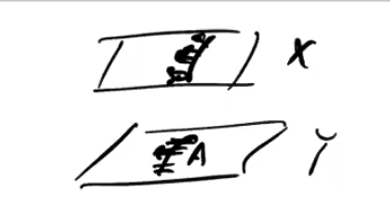
\includegraphics[width=3.64583in,height=\textheight]{figures/image_2020-11-15-01-41-25.png}
\caption{Image}
\end{figure}

\end{remark}

\begin{remark}

There are some equivalent definitions of a morphism being étale:

\begin{itemize}
\item
  Smooth of relative dimension zero
\item
  Locally finite presentation and \emph{formally étale}
\item
  Locally \emph{standard étale}, i.e.~for each \(x\in X\) with
  \(y\da f(x)\), there exists a \(U\ni x, V\ni y\) such that
  \(f(U) \subseteq V\) and \(V=\spec(R), U = \spec\qty{R[x]_h / g}\)
  (where we localize at \(h\)) such that the derivative \(g'\) is a unit
  in \(R[x]_h\) and \(g\) is monic.
\end{itemize}

For this last definition, thinking of \(\spec(R[x])\) as
\(R\times \AA^n\), what happens when modding out by a polynomial \(g\)?
This yields a curve cutting out the roots of \(g\). Inverting \(h\)
deletes the locus where \(h\) vanishes, and \(g'\) being a unit means
that the \(g\) has no double roots in the fibers. In other word, the
delete locus passes through all double roots:

\begin{figure}
\centering
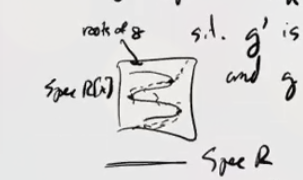
\includegraphics[width=3.64583in,height=\textheight]{figures/image_2020-11-15-01-47-05.png}
\caption{Image}
\end{figure}

\end{remark}

\begin{exercise}[?]

Check that standard étale morphisms are étale, and try to understand the
proof that all étale morphisms are locally standard étale.

\end{exercise}

Let's do some examples!

\begin{example}[Example of an étale morphism]

\envlist

\begin{itemize}
\item
  Multiplication by \([n]\) on an elliptic curve if \(n \in \ZZ\) is
  invertiable in the base field.
\item
  Take \(\GG_m = \spec k[t, t^{-1}]\), and the map
  \begin{align*}  
  \GG_m &\to \GG_m \\
   t^m &\mapsfrom t
  ,\end{align*} where \(n\) is prime to \(\ch(k)\).\footnote{Here we use
    the convention that everything is prime to zero.}

  \begin{itemize}
  \tightlist
  \item
    Note that this is in fact finite étale.
  \end{itemize}
\end{itemize}

\end{example}

\begin{exercise}[?]

Show that the last map above is étale. Hint: use the fact that
\(\dd{}{t} (t^n) = nt^{n-1}\), which is a unit.

\end{exercise}

\begin{example}[?]

Consider the map
\begin{align*}  
\GG_m &\injects \AA^1 \\
k[t, t^{-1}] &\mapsfrom k[t]
.\end{align*} We need to check 3 things:

\begin{itemize}
\tightlist
\item
  Locally finite presentation,

  \begin{itemize}
  \tightlist
  \item
    This is a finitely presented ring map, since you just need to adjoin
    an inverse of \(t\), one element and one relation.
  \end{itemize}
\item
  Flat,

  \begin{itemize}
  \tightlist
  \item
    Since open embeddings are flat,
  \end{itemize}
\item
  \(\Omega^1_{\GG_m / \AA^1} = 0\),

  \begin{itemize}
  \tightlist
  \item
    True for a Zariski open embedding.
  \end{itemize}
\end{itemize}

Note that this is finite onto its image.

\end{example}

\begin{proposition}[?]

Any open immersion is étale.\footnote{Note that we actually already
  checked this!}

\end{proposition}

\begin{example}[An étale morphism that is not finite onto its image]

Use the fact that \(\GG_m\) is \(\AA^1\sm\ts{\vector 0}\), so take
\(\GG_m \sm\ts{1}\) and the map
\begin{align*}  
\GG_m\sm\ts{1} &\to \GG_m \\
t^2 &\mapsfrom t
.\end{align*}

What's the picture? For the squaring map, there are two square roots:

\begin{figure}
\centering
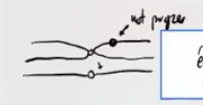
\includegraphics{figures/image_2020-11-15-02-01-04.png}
\caption{Image}
\end{figure}

This is an étale surjection but not finite étale, since it is not
proper. This also gives a counterexample to étale morphisms always
looking like covering spaces, since here that may be true locally but
doesn't hold globally.

\end{example}

\begin{warnings}

This is an important example to keep in mind, because you'll often see
arguments that treat étale maps as though they were finite onto their
image.

\end{warnings}

\begin{example}[?]

Take a finite separable field extension, taking \(\spec\) of it yields
an étale map.

\end{example}

Now for some non-examples:

\begin{example}[A finite map which is not etale]

Take \(X = \spec k[x, y] / xy\), which looks like the following:

\begin{figure}
\centering
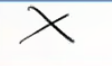
\includegraphics[width=3.64583in,height=\textheight]{figures/image_2020-11-15-02-04-46.png}
\caption{\(X\)}
\end{figure}

Then the normalization \(\tilde X\to X\) is not étale, since it is not
flat.

\end{example}

\begin{example}[A finite flat map which is not etale]

Take the map
\begin{align*}  
\AA^1 &\to \AA^1 \\
t^2 &\mapsfrom t
.\end{align*}

The picture is the following:

\begin{figure}
\centering
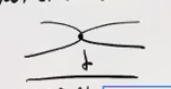
\includegraphics{figures/image_2020-11-15-02-07-04.png}
\caption{Image}
\end{figure}

This is note étale since it is ramified at zero. We can compute
\begin{align*}  
\Omega_f^1 = k[t]\, dt / d(t^2) = k[t] dt/ 2t\, dt
,\end{align*} where \(2t\,dt\) does not generate this module. This is
supported at \(t=0\) if \(\ch \neq 2\).

\end{example}

\begin{example}[?]

A finite flat morphism such that \(\Omega_{X/Y}^1\) is not torsion: a
hint is that the previous example almost works, with a slight
modification. Let \(\ch k = p\), and take
\begin{align*}  
\AA^1 &\mapsvia{F} \AA^1 \\
t^p &\mapsfrom t
.\end{align*} Then \(\Omega_f^1 = k[t]\, dt / d(t^p) = k[t]\,dt\) since
\(d(t^p) = 0\) in characteristic \(p\). This yields line bundles (?), so
it is not torsion.

\end{example}

\begin{remark}

This map has a name: the relative Frobenius. In general, looking at
Frobenii, the Kahler differentials will be very big. You might not be
used to this: in characteristic zero, a map of relative dimension zero
is generically étale. In this case, the Kahler differentials will always
be torsion.

\end{remark}

\begin{example}[?]

Consider a map
\begin{align*}  
\AA^m &\mapsvia{f_1, \cdots, f_m} \AA^m
,\end{align*} since such a map is given by a system of \(m\) polynomials
in \(m\) variables. Then \(f\) is étale is a neighborhood of
\(\vector a\) if \(\det \qty{\dd{f_i}{x_j} \evalfrom_{\vector a} }\) is
a unit.

\end{example}

\hypertarget{properties-of-uxe9tale-morphisms}{%
\subsubsection{Properties of Étale
Morphisms}\label{properties-of-uxe9tale-morphisms}}

\begin{proposition}[Some properties of étale morphisms]

\envlist

\begin{enumerate}
\def\labelenumi{\arabic{enumi}.}
\tightlist
\item
  Open immersions are étale
\item
  Compositions of étale morphisms are étale\footnote{What do you have to
    check? Locally finite presentation, flat, and unramified are all
    preserved. The one that may be tricky is remaining unramified, a
    hint is to use the cotangent exact sequence for \(\Omega^1_{X/Y}\).}
\item
  Base change of étale morphisms are étale, i.e.~

  \begin{center}\begin{tikzcd}
  X \cross_Y T\ar[d, "\therefore \text{étale}"']\ar[r] & X\ar[d, "\text{étale}"]  \\
  T\ar[r] &  Y\\
  \end{tikzcd}\end{center}
\item
  There is a 2 out of 3 property: If \(\phi \circ \psi\) and \(\phi\)
  are étale, then \(\psi\) is étale.
\end{enumerate}

\end{proposition}

\begin{exercise}[?]

Show property 4 above.

\end{exercise}

\begin{proposition}[?]

Étale morphisms on varieties over an algebraically closed field induce
isomorphisms on complete local rings at closed points.

\end{proposition}

\begin{exercise}[?]

Prove this! Hint: use the criterion for formal étaleness. There's an
evident map one way on local rings coming from your étale morphism, and
you need to produce the inverse map.

\end{exercise}

\begin{exercise}[?]

\(\danger\) If \(\psi\) is étale and \(\phi\circ\psi\) is étale, it is
not necessarily the case that \(\phi\) is étale. Come up with an
example!

\end{exercise}

\begin{corollary}[An informal statement]

Any property that can be checked at the level of complete local rings is
true for the source of an étale morphism if it is true for the target.

\end{corollary}

Why? If you want to check a property for complete local rings on the
source, note that the map induces an isomorphism of complete local
rings.

\hypertarget{generalizing-topologies}{%
\subsection{Generalizing Topologies}\label{generalizing-topologies}}

\hypertarget{sites}{%
\subsubsection{Sites}\label{sites}}

The notion of a \emph{site} will be a generalization of topological
spaces and sheaves. The idea is we'll generalize sheaf cohomology to
this setting. On a nice space like a manifold, singular cohomology is
isomorphic to the sheaf cohomology of the constant sheaf
\(\underline{\ZZ}\). Here we'll find some version of a sheaf where étale
cohomology with \(\ZZ/\ell^n\ZZ\) coefficients will be the sheaf
cohomology with the constant sheaf \(\underline{\ZZ/\ell^n\ZZ}\).

\begin{question}

What parts of the definition of a topological space are needed to define
the notion of a sheaf?

\end{question}

\begin{remark}

Recall that the \emph{sheaf condition} is given in two parts:

\begin{enumerate}
\def\labelenumi{\arabic{enumi}.}
\item
  A section is determined by its value on a cover, and
\item
  Sections can be glued when they agree on intersections.
\end{enumerate}

\end{remark}

\begin{answer}

\envlist

\begin{enumerate}
\def\labelenumi{\arabic{enumi}.}
\tightlist
\item
  As in presheaves, a notion of open sets and inclusions. (I.e., a
  category of open sets.)\footnote{Recall that a presheaf on \(X\) is a
    contravariant functor out of the category of open sets of \(X\).}\footnote{The
    notion of a presheaf on \(X\) doesn't know much about the actual
    topology of \(X\). If two spaces have the coarsest topology, so the
    only opens are \(X, \emptyset\), then the categories of open sets
    are equivalent, and every presheaf on them will be the same.}
\end{enumerate}

We'd also like to make sense of the sheaf condition:

\begin{enumerate}
\def\labelenumi{\arabic{enumi}.}
\setcounter{enumi}{1}
\item
  Collections of morphisms which are ``covers'', remembering which
  collections of opens cover a space, and
\item
  The existence of certain fiber products (intersections).
\end{enumerate}

\end{answer}

\begin{remark}

The motivation for (3) above is that for \(U, V \subseteq X\), we can
form \(U\cross V = U\intersect V\).

\end{remark}

\begin{definition}[Preliminary: Sites/Grothendieck Topologies]

A category \(\mathcal{C}\) with a collection of \emph{covering families}
\(\ts{X_\alpha \mapsvia{f_\alpha} X \st \alpha\in A}\)\footnote{How to
  think of this: elements in this collection cover \(X\).} such that
several axioms are satisfied.

\end{definition}

We'll discuss the axioms next time, they just capture the notion of what
a cover of a topological space should look like.

\begin{warnings}

There are at least three different notions of this definition! The one
above is perhaps the least general but the easiest to work with.

\end{warnings}

\begin{example}[?]

For \(X\) a topological space, \(\mathcal{C}\) the category of open sets
in \(X\), then \(\ts{U_\alpha\to U}\) is a covering family if the
\(U_\alpha\) cover \(U\), i.e.~\(U = \union_\alpha U_\alpha\).

\end{example}

\begin{example}[More exotic]

Let \(M\) be a manifold and \(\mathcal{C}\) be the category of manifolds
over \(M\), so all \(M' \mapsvia{f} M\) such that \(f\) is locally an
isomorphism. Note that these are smooth local homeomorphisms. Let
\(\ts{M_\alpha \mapsvia{f_\alpha} M}\) if
\(\union_\alpha \im (f_\alpha) = M\).

\end{example}

\begin{example}[Another exotic example]

Let \(X\) be a scheme and consider \(X_{\text{et}}\) the category of all
étale \(Y/X\): so the objects are schemes \(Y\) admitting an étale
morphism \(Y\to X\). Then \(\ts{X_\alpha\to X}\) is a covering family if
\(\union \im (f_\alpha) = X\).

\end{example}

This will be the fundamental object, and we'll define étale cohomology
by defining sheaves on this category, taking a constant sheaf
\(\underline{\ZZ/\ell^n\ZZ}\), and we'll take sheaf cohomology.

\hypertarget{lecture-3}{%
\section{Lecture 3}\label{lecture-3}}

\hypertarget{defining-sites}{%
\subsection{Defining Sites}\label{defining-sites}}

Today: we'll discuss sites, which generalizes the category of open sets
over a topological space. The goal is to generalize spaces and sheaves
to categories, and to define a sheaf we need

\begin{enumerate}
\def\labelenumi{\arabic{enumi}.}
\item
  A notion of a \emph{cover}, and
\item
  A notion of intersections/fiber products of open sets.
\end{enumerate}

\begin{definition}[Grothendieck Topology / Sites]

A \textbf{Grothendieck topology} on \(\mathcal{C}\) or a \textbf{site}
on \(\mathcal{C}\) is the data of for each
\(X\in \mathrm{Ob}(\mathcal{C})\) a collection of sets of morphism
\(\ts{X_\alpha \to X}\) (\emph{covering families}) satisfying

\begin{itemize}
\item
  Intersections exist: If \(X_\alpha\to X\) appears in a covering family
  and \(Y\to X\) is arbitrary, the fiber product \(X_\alpha\cross_X Y\)
  exists.
\item
  Intersecting with a cover again yields a cover: If
  \(\ts{X_\alpha\to X}\) is a covering family and \(Y\to X\) is
  arbitrary, then the covering family can be pulled back:
  \(\ts{Y\cross_X X_\alpha\to Y}\) is again a covering
  family.\footnote{When \(\mathcal{C}\) was the category of open sets of
    a space \(X\), the existence of this morphism \(Y\to X\) says
    \(Y \subseteq X\) is an open subset, and thus intersecting \(Y\)
    with any open cover of \(X\) yields an open cover of \(Y\).}
\item
  Compositions of coverings are again coverings: If
  \(\ts{X_\alpha\to X}_{\alpha}\) and
  \(\ts{X_{\alpha\beta} \to X_\alpha}_{\alpha,\beta}\) are covering
  families, then you can compose, i.e.~taking the set of all possible
  ways of composing \(\ts{X_{\alpha\beta} \to X_\alpha \to X}\) is again
  a covering family.\footnote{For spaces, this says if you have a cover
    of an open set by subsets and a cover of each of those subsets, the
    entire set has been covered.}
\item
  Isomorphisms are covers: If \(X\mapsvia{\sim_f} Y\) is an isomorphism,
  then the singleton family \(\ts{X\mapsvia{f} Y}\) is a covering
  family.
\end{itemize}

\end{definition}

\hypertarget{examples-of-sites}{%
\subsubsection{Examples of Sites}\label{examples-of-sites}}

\begin{example}[The motivating example]

If \(X\) is a topological space, define \(\mathcal{C}\) whose objects
are open subsets of \(X\) where there is a unique morphism \(U\to V\)
iff \(U\subseteq V\). Then \(\ts{U_\alpha \to U}\) is a covering family
if \(\Union_\alpha U_\alpha = U\).

\end{example}

\begin{example}[The small étale site]

Let \(X\) be a scheme, and define the small étale site \(X_{\et}\): the
category whose objects are étale morphisms \(Y\mapsvia{f} X\) where
morphisms are maps over \(X\):

\begin{center}\begin{tikzcd}
Y_1 \ar[rd, "{f_1}"]\ar[rr, "g"] & & Y_2\ar[ld, "{f_2}"] \\
 & X & 
\end{tikzcd}\end{center}

Note that \(g\) is étale by the 2 out of 3 property.

Then \(\ts{X_\alpha\to X}\) is a covering family if the set theoretic
images satisfy \(\Union_\alpha \im(f_\alpha) = X\).

\end{example}

\begin{example}[The big étale site]

Again let \(X\) be a scheme, and define \(X_{\mathrm{Et}}\) the category
whose objects are all \(X\dash\)schemes (where we no longer require the
maps to be étale). In other words, this is the overcategory of \(X\):
the category of schemes over \(X\). Then
\(\ts{U_\alpha\mapsvia{f_\alpha}U}\) is a covering family if all of the
\(f_\alpha\) are étale and \(\Union_\alpha \im(f_\alpha) = U\).

\end{example}

Note the difference: in the small site, we included only étale
\(X\dash\)schemes, vs all \(X\dash\)schemes in the big site. In both
cases, the notion of covering families are the same.

\begin{example}[?]

Let \(X\) be a complex analytic space (e.g.~a complex manifold), then
there is an analytic étale site whose objects are complex analytic
spaces \(Y\mapsvia{f} X\) such that locally on \(Y\), \(f\) is an
analytic isomorphism. Note that this includes covering spaces. The
morphisms will be morphisms over \(X\) creating commuting triangles, and
the covers are the usual covers.

\end{example}

\begin{remark}

This category is part of what motivates the definition of the étale
topology. This is what we're trying to imitate. E.g. if you have a
complex algebraic variety, taking its analytification will be one of
these. This site will show up later when we compare étale cohomology to
singular cohomology.

\end{remark}

\begin{remark}

We haven't said what it means to be a sheaf yet, but Grothendieck
topologies behave in somewhat unexpected ways. The category of sheaves
of the analytic étale cohomology, \(\Sh(X_{\mathrm{an\dash et}})\), is
canonically equivalent to \(\Sh(X^{\mathrm{top}})\). Thus sometimes the
category of sheaves over a site doesn't remember the site, i.e.~two
different sites can have the same category of sheaves. On the RHS we had
a category of open subsets, whereas on the LHS we included things like
covering spaces. We'll see later that there is a notion of morphisms of
sites, and there is a morphism inducing this equivalence.

Proving this isomorphism will be an exercise, here's an outline of why
it's true: suppose you have a cover of \(X\) in this category, i.e.~a
family of local analytic isomorphisms. Given any of these, you can cover
by subsets for which these are isomorphisms onto their images.

\end{remark}

\begin{example}[The fppf topology]

This stands for \textbf{faithfully flat and finite presentation}.
\footnote{The letters don't precisely match up here because this comes
  from a French acronym.} There are small and big sites here: we define
\(X_{\fppf}\) whose objects are fppf morphism \(Y\to X\), with morphisms
as triangular diagrams of morphisms over \(X\), and covers are the usual
covers. Note that replacing fppf morphisms with flat morphisms would
yield an equivalent definition here.

\end{example}

\begin{example}[?]

If \(X\) is a scheme, then the small Zariski topology is
\(X_{\mathrm{zar}}\) whose objects are \(\Op(X^{\mathrm{top}})\), the
Grothendieck topology of the corresponding topological space, and we
take the usual notion of covers.

There is a big Zariski topology \(X_{\mathrm{Zar}}\) whose category is
all \(X\dash\)schemes \(\ts{U_\alpha\mapsvia{f_\alpha} U}\) with
\(f_\alpha\) open embeddings and \(\Union_\alpha \im(f_\alpha) = U\).

\end{example}

\begin{example}[?]

Some other examples:

\begin{itemize}
\item
  The \textbf{Nisnevich} topology, which lives between the Zariski and
  the étale topology,
\item
  The \textbf{crystalline} site, used to define crystalline cohomology,
\item
  The \textbf{infinitesimal} site,
\item
  The \textbf{cdh} topology, the \textbf{arc} topology, the \textbf{rh}
  topology, and many more.
\end{itemize}

\end{example}

\hypertarget{toward-sheaves-of-sites}{%
\subsection{Toward Sheaves of Sites}\label{toward-sheaves-of-sites}}

\begin{definition}[Presheaf]

For \(\mathcal{D}\) a category, a \(\mathcal{D}\dash\)valued presheaf is
a contravariant function \(F:\mathcal{C}\to \mathcal{D}\).

\end{definition}

\begin{remark}

This makes no reference to any Grothendieck topology.

\end{remark}

\begin{example}[?]

If \(X\) is a topological space, a \(\mathcal{D}\dash\)valued presheaf
of \(X\) is equivalent to a presheaf on \(\Op(X)\).

\end{example}

We can now define a sheaf. What's the motivation? For \(X\) a
topological space, it's a sheaf satisfying some conditions: its sections
are determined by an open cover, and given sections agreeing on overlaps
allows gluing. This can be captured by a specific diagram, which is what
we will use here.

Recall that a site is a category equipped with the Grothendieck
topology.

\begin{definition}[Sheaf]

A sheaf \(F\) is presheaf such that

\begin{center}\begin{tikzcd}
F(U) \ar[r] & \prod_\alpha F(U_\alpha) \ar[r, shift left=0.75ex, "F(\pi_1)"] \ar[r, shift right=0.75ex, "F(\pi_2)"'] & \prod_{\alpha, \alpha'} F(U_\alpha \cross_U U_{\alpha'}) 
\end{tikzcd}\end{center}

is an \emph{equalizer} diagram for all covering families
\(\ts{U_\alpha \to U}\).

\end{definition}

\begin{remark}

The diagram arises due to the fact that if we have a bunch of maps
coming from a cover, since we have a contravariant functor, we get a map
into the product. We then look at the intersections of all
\(U_{\alpha}, U_{\alpha'}\).

The two arrows occurring come from the projections:

\begin{center}\begin{tikzcd}
& U_\alpha \cross_U U_{\alpha'} \ar[dl, "\pi_1"] \ar[rd, "\pi_2"] & \\
U_\alpha\ar[dr, hook] & & U_{\alpha'}\ar[dl, hook] \\
& U &
\end{tikzcd}\end{center}

where we use the fact that since \(F\) is a contravariant functor, it
induces maps going the other way.

What does being an equalizer mean, say if \(F\) is set-valued?
``Exactness'' at the middle term is the gluing condition, and exactness
at the first term is injectivity, i.e.~a section (the values of \(F\) on
\(U\)) are determined by its values on a cover (by \(F(U_\alpha)\)).
Note that in fact \(F(U)\) is the limit of this diagram. The gluing
condition is more precisely that if we're given
\((s_\alpha) \in \prod_\alpha F(U_\alpha)\) such that
\(F(\pi_1)(s_\alpha) = F(\pi_2)(s_\alpha)\), then \((s_\alpha)\) comes
from \(F(U)\).

\end{remark}

\begin{definition}[Morphisms of sheaves and presheaves]

A morphism \(F_1\to F_2\) of either presheaves or sheaves is a natural
transformation of functors.

\end{definition}

\hypertarget{examples-of-sheaves-of-sites}{%
\subsubsection{Examples of Sheaves of
Sites}\label{examples-of-sheaves-of-sites}}

\begin{theorem}[?]

Any representable functor is a sheaf on the étale site \(X_{\Et}\). In
fact, any such functor is a sheaf on the big fppf site \(X_{\Fppf}\):
the category of all \(X\dash\)schemes with covers as fppf covers, which
are maps that are flat and jointly surjective.

\end{theorem}

\begin{example}[Examples of sheaves on the étale site]

Take \(\mu_n\) the functor represented by
\(\mu_n \da \spec k[t] / t^{n-1}\). For \(U\) an \(X\dash\)scheme, we
can evaluate in the following way:
\begin{align*}  
\mu_n(U) = \ts{f\in \OO_U(U) \st f^n = 1}
.\end{align*}

\end{example}

\begin{example}[?]

We define a sheaf of the étale site as \(\OO^{\et}_X(U) = \OO_U(U)\)
where we've said what the values are. This is a sheaf that is
represented by \(\AA^1_{/X}\).

\end{example}

\begin{example}[?]

The constant sheaf \(\underline{\zlnz}\). How can we prove it is a
sheaf, given the theorem, and determine what its values are? This is
represented by \(\qty{\zlnz} \cross X\), i.e.~taking the disjoint union
of \(\ell^n\) copies of \(X\). The values are given by
\begin{align*}  
\underline{\zlnz}(U) =  \hom_{\Top}(U^{\Top}, \zlnz)
,\end{align*} where we give the set \(\zlnz\) the discrete topology and
take morphisms to be continuous maps.

\end{example}

\begin{warnings}

The constant sheaf \(\underline{S}\) doesn't associate \(S\) to every
open set: it instead associates \(S^d\) where \(d\) is the number of
components. The former would only be a presheaf, and not a sheaf.

\end{warnings}

\begin{example}[?]

We can take the sheaf \(\GG_m(U) \da \OO_U(U)\units\), whose values are
obtained by taking the global sections of the structure sheaf and only
keeping the units. This is represented by
\begin{align*}
\GG_{m, X} = \spec \ZZ[t, t^{-1}] \fp{\spec \ZZ} X
\end{align*} Why does this represent this functor? Mapping into this
requires that \(t\) goes to an invertible function, which yields the
isomorphism.

\end{example}

\begin{remark}

Note that all of these functors take values in abelian groups, which is
a consequence of the fact that the representing objects are group
schemes. In fact, one definition of a group scheme is that the functor
it represents factors through groups.

\end{remark}

\begin{example}[?]

Take the functor \(\PP^n(U) \da \hom(U, \PP^n)\). This functor can be
written down as a line bundle on \(U\) with a surjective map from
\(\OO_U \to \OO_U^n\) (?), the functor represented by projective space,
and that's also a sheaf that is necessarily representable but not an
abelian one.

\end{example}

Some things we still need to get to:

\begin{itemize}
\tightlist
\item
  A proof that \(\ul{zlnz}\) is actually a sheaf,
\item
  A proof that the category of sheaves on the big étale site
  \(X_\Et\)\footnote{Note that a sheaf on the big étale site necessarily
    restricts to a sheaf on the small étale site, since covers in the
    small site are also covers in the big site.} with values in
  \(\thecat{Ab}\) is abelian and has enough injectives.
\end{itemize}

\hypertarget{uxe9tale-cohomology-a-preliminary-definition}{%
\subsection{Étale Cohomology: A Preliminary
Definition}\label{uxe9tale-cohomology-a-preliminary-definition}}

\begin{definition}[Imprecise: étale cohomology]

Let \(\mathcal{F}\) be a sheaf and define a functor
\(\Gamma_X: \mathcal{F}\to \mathcal{F}(X)\) sending it to its values on
\(X\). Then
\begin{align*}  
H^i(X_\et, \ul{\zlnz}) \da R^i \Gamma_X(\ul \zlnz)
,\end{align*} the right-derived functors of \(\Gamma_X\).

\end{definition}

\begin{remark}

This definition is incomplete, and in particular, it's highly
non-obvious that this category of abelian sheaves is abelian. E.g.
usually when proving that the category of abelian sheaves on a
topological space has cokernels, you use sheafification: you take the
cokernel of a map of presheaves, which is a presheaf, and sheafify it.
Here, we don't know how to sheafify a presheaf on a site. The usual
construction involves forming the \emph{espace étalé} and taking
sections does not work for a site, you need a genuinely different
argument.

\end{remark}

\begin{warnings}

Even showing cokernels exist in the category of abelian sheaves on a
site is nontrivial. Try as an exercise!

\end{warnings}

\begin{remark}

What will be true in general is that this category will be an \(AB5\)
abelian category, and having enough injectives is all that's
additionally needed. This comes from machinery developed in
Grothendieck's Tohoku paper, and we'll sketch part of the proof.

\end{remark}

Properties of these sheaves are not so obvious, and depend on the site
you're working over:

\begin{example}[?]

Consider the map
\begin{align*}  
\GG_m &\to \GG_m \\
t^m &\mapsfrom t
,\end{align*} where \(n\) is invertible over the base, e.g.~if we're
over a field of characteristic coprime to \(n\). This yields a map of
sheaves in two different settings. In \(X_{\mathrm{Zar}}\) we have
\begin{align*}  
\OO\units &\to \OO\units \\
f &\mapsto f^n
.\end{align*}

We can look at this in \(X_{\et}\), yielding
\begin{align*}  
\OO_\et\units &\to \OO_\et\units \\
f &\mapsto f^m
.\end{align*}

\begin{claim}

This map is not an epimorphism on \(X_{\mathrm{Zar}}\) but is on
\(X_{\et}\)

\end{claim}

\begin{proof}[?]

It suffices to give one example: take \(X = \spec \RR\) and \(n=2\), and
since this is just a point, the sheaf is determined by its values. So is
the map
\begin{align*}  
\RR\units &\to \RR\units \\
t &\mapsto t^2
\end{align*} surjective? The answer is no, of course, since its image is
\(\RR_{\geq 0}\).

This will be surjective on \(X_{\et}\) if \(n\) is invertible on \(X\).
If we were in usual topological spaces, we would want to show that given
any section of the sheaf on an open set, it can be refined. Here we want
to pass to an étale cover so that section has an \(n\)th root. So given
\(f\in \GG_m(U)\), we want an étale cover of \(U\) so that \(f\) obtains
an \(n\)th root. An invertible function is a map \(U\to \GG_m\), and we
can form the square

\begin{center}\begin{tikzcd}
 U \fp{\GG_m} \GG_m\ar[r]\ar[d] & \GG_m & z^m  \ar[d] \\
 U\ar[r] &  \GG_m & z\ar[u, |->]
\end{tikzcd}\end{center}

The RHS map is étale since \(n\) is invertible, and the fiber product is
étale since étale morphisms are preserved by base change.

\begin{claim}

\(f\) has an \(n\)th root upstairs. (Verify!)

\end{claim}

There's a more concrete way of writing this: note that
\(\AA^1_{U, z} = \spec k[t]\), so take the subscheme cut out by
\(V(z^n - f)\). This will be an étale cover of \(U\) (the same one in
fact) and \(z\) is now an \(n\)th root.

\end{proof}

\end{example}

\begin{exercise}[?]

Check the details! Namely that this argument implies that this map of
sheaves is an epimorphism.

\end{exercise}

\begin{remark}

This map of sheaves \(\GG_m \mapsvia{z^m \mapsfrom z} \GG_m\), noting
that if \(n\) is not invertible this will not be an epimorphism, will
always be an epimorphism in \(\Sh(X_\fppf)\) since this map is flat and
finitely presented.

\end{remark}

\hypertarget{preview-morphisms-of-sites}{%
\subsection{Preview: Morphisms of
Sites}\label{preview-morphisms-of-sites}}

\begin{definition}[Morphisms of Sites]

Suppose \(T_1, T_2\) are sites (categories with covering families), then
a continuous map \(f:T_1 \to T_2\) is a functor
\(T_2 \to T_1\)\footnote{Note that this functor goes in the opposite
  direction of the original map.} that preserves fiber products and
sends covering families to covering families.

\end{definition}

\begin{example}[?]

A continuous map \(f\in \Hom_\Top(X, Y)\) induces a map
\begin{align*}  
\Op(Y) &\to \Op(X) \\
U &\mapsto f^{-1}(U)
.\end{align*}

\end{example}

\begin{exercise}[?]

Check that this is a continuous map of sites.

\end{exercise}

Next time: a bunch of examples.

\section{Indices}
\listoftodos[List of Todos]
\newpage

% Hook into amsthm environments to list them.
\renewcommand{\listtheoremname}{Definitions}
\listoftheorems[ignoreall,show={definition}, numwidth=3.5em]

\renewcommand{\listtheoremname}{Theorems}
\listoftheorems[ignoreall,show={theorem,proposition}, numwidth=3.5em]

\renewcommand{\listtheoremname}{Exercises}
\listoftheorems[ignoreall,show={exercise}, numwidth=3.5em]

\listoffigures


\printbibliography[title=Bibliography]


\end{document}
